%%%%%%%%%%%%%%%%%%%%%%%%%%%%%%%%%%%%%%%%%%%%%%%%%%%%%%%%%%%%%%%%%%%%%%%%%%%%%%%%
%2345678901234567890123456789012345678901234567890123456789012345678901234567890
%        1         2         3         4         5         6         7         8

%\documentclass[letterpaper, 10 pt, conference]{ieeeconf}  % Comment this line out if you need a4paper

\documentclass[letterpaper, 10pt, conference]{IEEEconf}      % Use this line for a4 paper

\IEEEoverridecommandlockouts                              % This command is only needed if 
                                                          % you want to use the \thanks command

\overrideIEEEmargins                                      % Needed to meet printer requirements.

% See the \addtolength command later in the file to balance the column lengths
% on the last page of the document

% The following packages can be found on http:\\www.ctan.org
\usepackage{graphics} % for pdf, bitmapped graphics files
\usepackage{epsfig} % for postscript graphics files
\usepackage{mathptmx} % assumes new font selection scheme installed
\usepackage{times} % assumes new font selection scheme installed
\usepackage{amsmath} % assumes amsmath package installed
\usepackage{amssymb}  % assumes amsmath package installed
\usepackage[acronym]{glossaries}
\usepackage{subfiles}
% new added
%\usepackage{fixltx2e}
%\usepackage{dblfloatfix}
%\usepackage{geometry}% http://ctan.org/pkg/geometry
%\usepackage{lipsum}% http://ctan.org/pkg/lipsum
\usepackage{siunitx}
\usepackage{graphicx}
\usepackage{epstopdf}
\usepackage{tikz}
\usepackage{hyperref}
\usepackage{bookmark}
\makeglossaries

%\renewcommand\@seccntformat[1]{}

\usetikzlibrary{arrows,positioning,shapes.geometric}

\DeclareGraphicsExtensions{.eps}
\subfile{glossary}

\title{\LARGE \bf
Development and evaluation of an experimental platform for steered axles of long combination vehicles}

\author{Michael Hofmann$^{1}$ and Sebastian Franz$^{1}$% <-this % stops a space
	%\thanks{*This work was supported by Volvo Group Trucks Technology, Chalmers University of Technology, SAFER, Parator.}% <-this % stops a space
	\thanks{$^{1}$Vehicle Engineering and Autonomous Systems, Department of Applied Mechanics, Chalmers University of Technology, SE-412~96 G\"OTEBORG, Sweden,
		{\tt\small michael.hofmann@alumni.chalmers.se},
		{\tt\small sebastian.franz@alumni.chalmers.se}}%
}





\begin{document}



\maketitle
\thispagestyle{empty}
\pagestyle{empty}


%%%%%%%%%%%%%%%%%%%%%%%%%%%%%%%%%%%%%%%%%%%%%%%%%%%%%%%%%%%%%%%%%%%%%%%%%%%%%%%%
\begin{abstract}

\gls{HCT}-vehicles require different strategies in controlling lateral dynamics of the combinations to ensure optimal paths taken by the trailers. These steering algorithms have been developed in previous works and now need to be verified on the track. This work thus implemented a dolly experimentation platform incorporating a rapid-prototyping system to provide the possibility of evaluating these algorithms. The solution is detailed as a \gls{HIL}-test linked with a vehicle dynamics frame-work in this publication. Results for this setups utilizing the aforementioned algorithms are presented and discussed. Nevertheless it is possible to run the outlined solution on-track, for which some suggestions are given at the end of this work.

\end{abstract}


%%%%%%%%%%%%%%%%%%%%%%%%%%%%%%%%%%%%%%%%%%%%%%%%%%%%%%%%%%%%%%%%%%%%%%%%%%%%%%%%
\section{Introduction}

The driving behaviour of \gls{HCT} vehicles is in many ways different to that of single unit trucks and needs to be researched in great detail to gain an understanding of the vehicle's dynamic properties, that is equally detailed as it is for other vehicle classes. This will lead to development of better safety and assistance systems and thus reduce threat potential, accidents and fatalities involving this emerging mode of transportation. 

The research project in which this thesis is embedded aims to develop an active dolly, meaning that steering will be autonomously conducted by the dolly based on the driving situation at hand and various vehicle parameters (e.g. speed, steering wheel angle).
This abstract control algorithm will be executed on a rapid-prototyping system which is linked to and controls the dolly. To supply this connection between the hardware and control-algorithm implemented in the modeling-environment Simulink is the main-contribution of this work. 


The following points will be covered in this paper:
\begin{itemize}
\item hardware and software utilized to achieve \gls{HIL} verification for an active converter dolly
\item evaluation of existing delays in the implementation and their consequences
\item discussion of three standard maneuvers for \gls{HCT}-combinations executed on the  developed \gls{HIL}-system using the aforementioned controllers and a comparison with simulation results
\item propose necessary changes to the set-up for taking the developed solution to the test-track in the future
\end{itemize}


\section{Hardware-setup}

\subsection{Base vehicle}

The hardware base is a dolly manufactured by Parator Industries. The steering system is based around the \gls{ETS} developed and built by \gls{VSE} with two hydraulically steerable axles. It was originally meant to be used in trailer steering and as an after-market system does not tie in with any of the truck's communication networks or sensor data. This makes it OEM-independent and very robust. The \gls{ETS} solely relies on the articulation angle between the leading and following unit on which the system is mounted and the speed of the combination. The articulation angle is gathered via a dedicated sensor mounted on the king-pin, the speed-signal is gathered from the ISO-11992 \gls{CAN}.

\subsection{Rapid-prototyping system (\gls{MABII})}

To execute the readily developed algorithms\cite{c27}, that govern the steering of the \gls{HCT}-combination needed to be ported to a platform, capable of interacting with the dolly and the tractor, while ensuring robust behavior during run-time. It was decided to incorporate the \gls{MABII} by dSpace, a real-time platform for its advantages in automotive environments with a vast selection of in- and outputs for interfacing with vehicular communications systems (\gls{CAN}, ethernet, FlexLink). It conveniently ties in with Simulink, which was used for algorithm development, for code-generation. Furthermore it physically is very robust and has good logging possibilities.


\subsection{Arduino}

To convert from \gls{CAN}-messages to serial output an Arduino Due together with a MCP2551 \gls{CAN}-transceiver was used. This provided the feedback-loop from the hardware-system to the simulation environment during the \gls{HIL}-testing.

\subsection{interconnections between MABII/dolly/truck}


\section{Software-setup} 

In this section a short overview of the utilized software and its interdependencies shall be given. 

\subsection{\gls{VTM}}

To evaluate the dynamic performance of the \gls{HCT}-combination Volvo's \gls{VTM} came to use. It is a library developed in and for Simulink and permits the simulation of truck dynamics based on a multi-body model for the kinematic relation and a parametrized tire model around the magic formula. Many different \gls{HCT}-combinations, road-situations and maneuver definitions come pre-defined with the tool-kit enabling a fairly quick implementation of full vehicle simulations. 

\subsection{RTI-blockset}

dSpace's rapid-prototyping platform's connection with Simulink is centered around a library which provides access to all physical communication ports on the \gls{MABII}, real-time execution on the target hardware and straight forward code-generation and -download. It was used to implement the \gls{CAN}-communication with the \gls{ETS}, the \gls{EBS} and will be used to incorporate more signals from the truck's chassis-\gls{CAN} in the future. Another use of the block-set was to ensure \gls{UDP}-communication within the \gls{HIL}-testing, as the Ethernet-port on the \gls{MABII} was used to supply data from the hardware system to the simulated sub-systems.

\subsection{ControlDesk}

As the simulation is executed on the \gls{MABII} it is possible to access representations of all blocks and their values and properties that are part of the abstract Simulink model which was generated to the \gls{MABII}. It thus is possible to have a user-readable system-state monitor. A number of \gls{GUI} creation tools permit fast development. During execution ControlDesk runs on a standard PC, which accesses the \gls{MABII}'s RAM via ethernet connection. 

%\begin{figure}
%\centering
%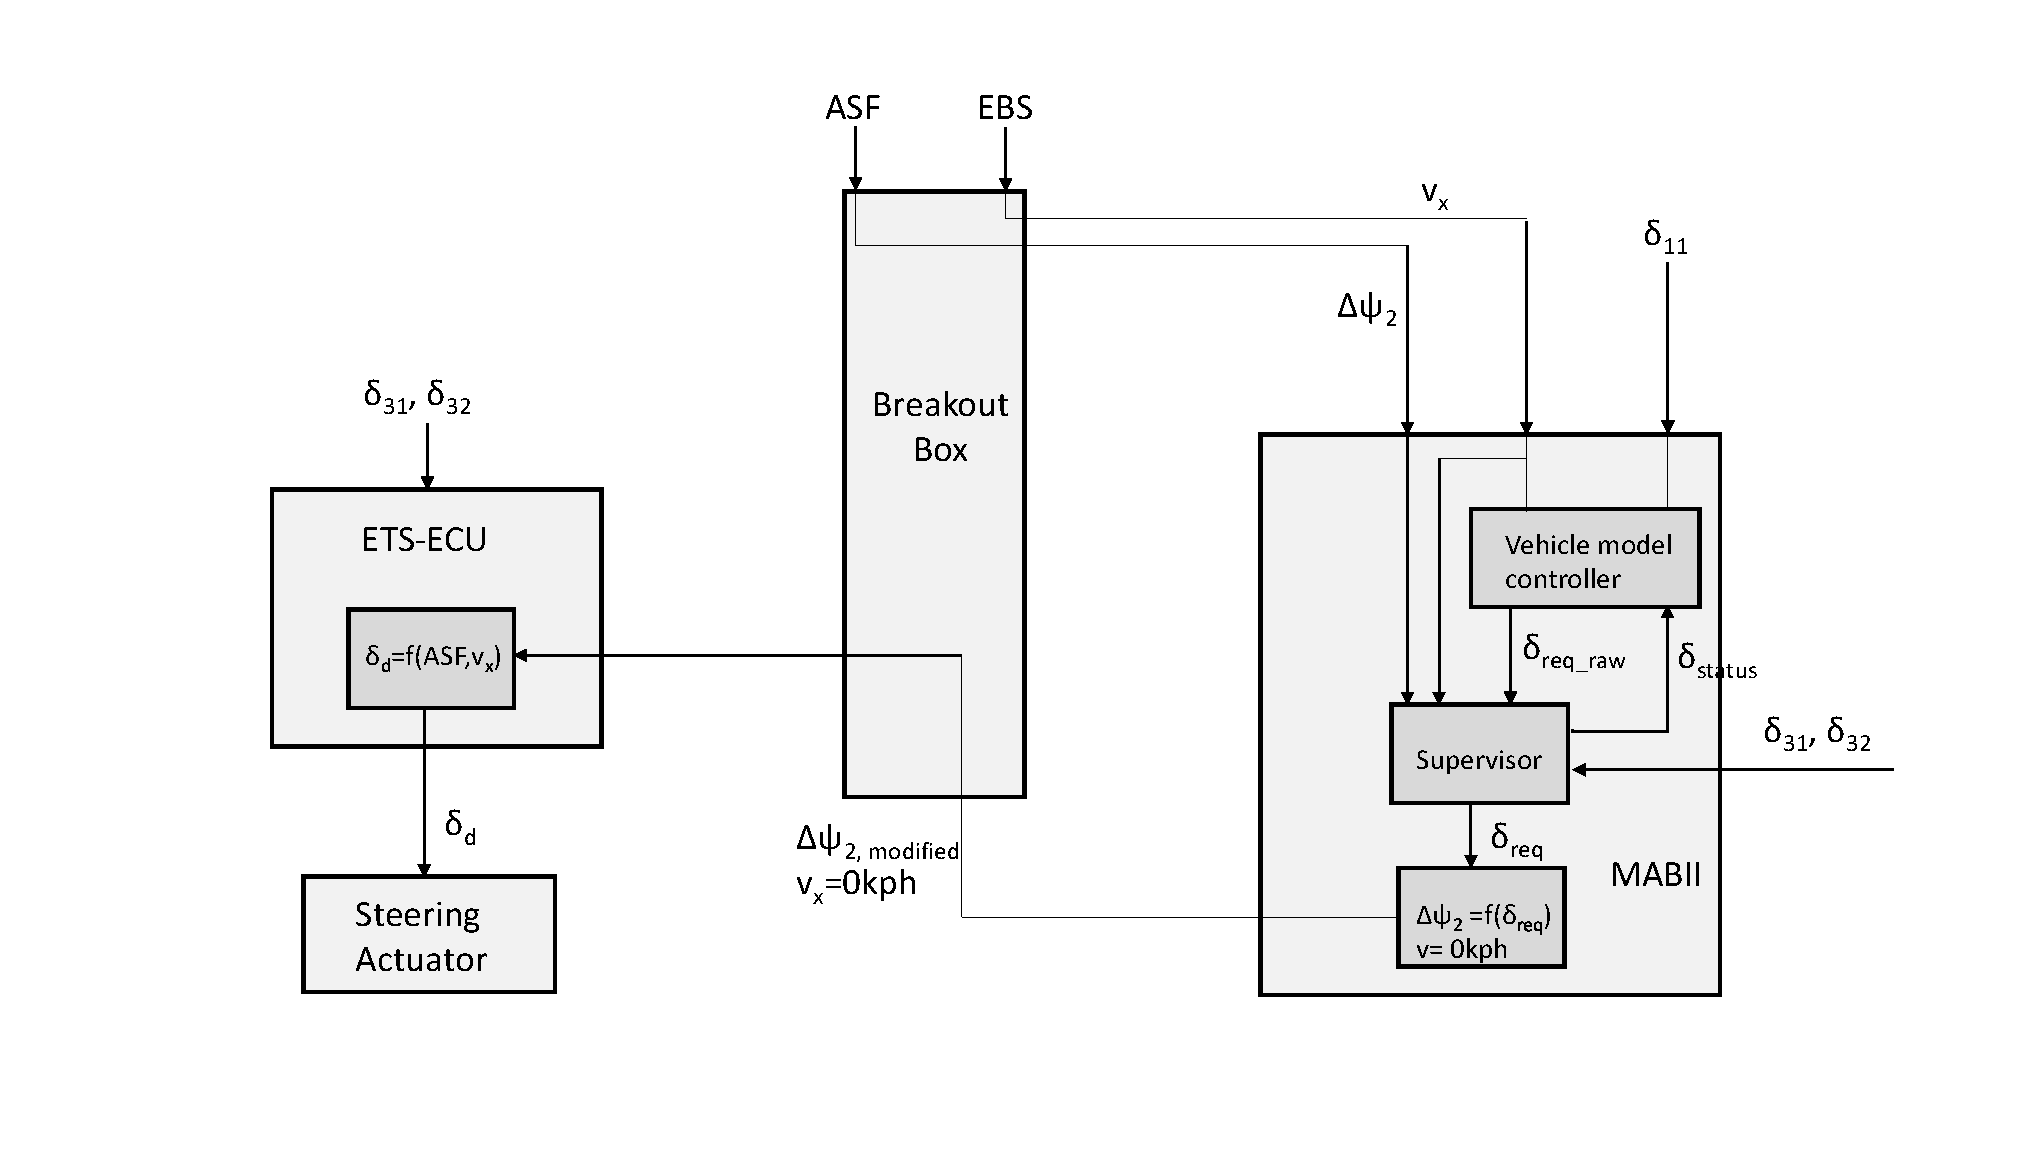
\includegraphics[width=1\linewidth]{system_mod}
%\caption{Signal path overview for modified \gls{ETS}}
%\label{fig:system_mod}
%\end{figure}

\section{\gls{HIL}-architecture}
\gls{VTM} includes a lot of processing-heavy sub-models (tire models, vehicle parameter sets) which lead to processing power not sufficing to allow for \gls{VTM}'s execution in the dSpace environment on the \gls{MABII}. To perform \gls{HIL}-testing it was thus necessary to split the computational load and accomplish real-time data exchange between the hardware controlling-system on the \gls{MABII} and the rest of the simulation which will be run parallely in Simulink in real-time on a standard PC. Though there are dedicated real-time platforms available to achieve real-time execution it was decided to rely on a standard PC to minimize costs and have a lean work-process without extra steps of code conversion to different platforms. Figure \ref{fig:HIL_overview} illustrates the distribution of the \gls{HIL}-setup's different components according to the Volvo GTT functionality model over two computers, the \gls{MABII} and the actual hardware. The \gls{VMM} consists of the controller previously developed which is executed on the Simulation-PC and the steering interface executed on the \gls{MABII}. For track-testing it of course is necessary to also port the controller for execution on the \gls{MABII} to have one closed of system. This was not yet possible to achieve for the tests at hand, as some blocks used within the controller-algorithm's  Simulink were incompatible for real-time execution on the dSpace system.

\begin{figure*}[h]
	\centering
	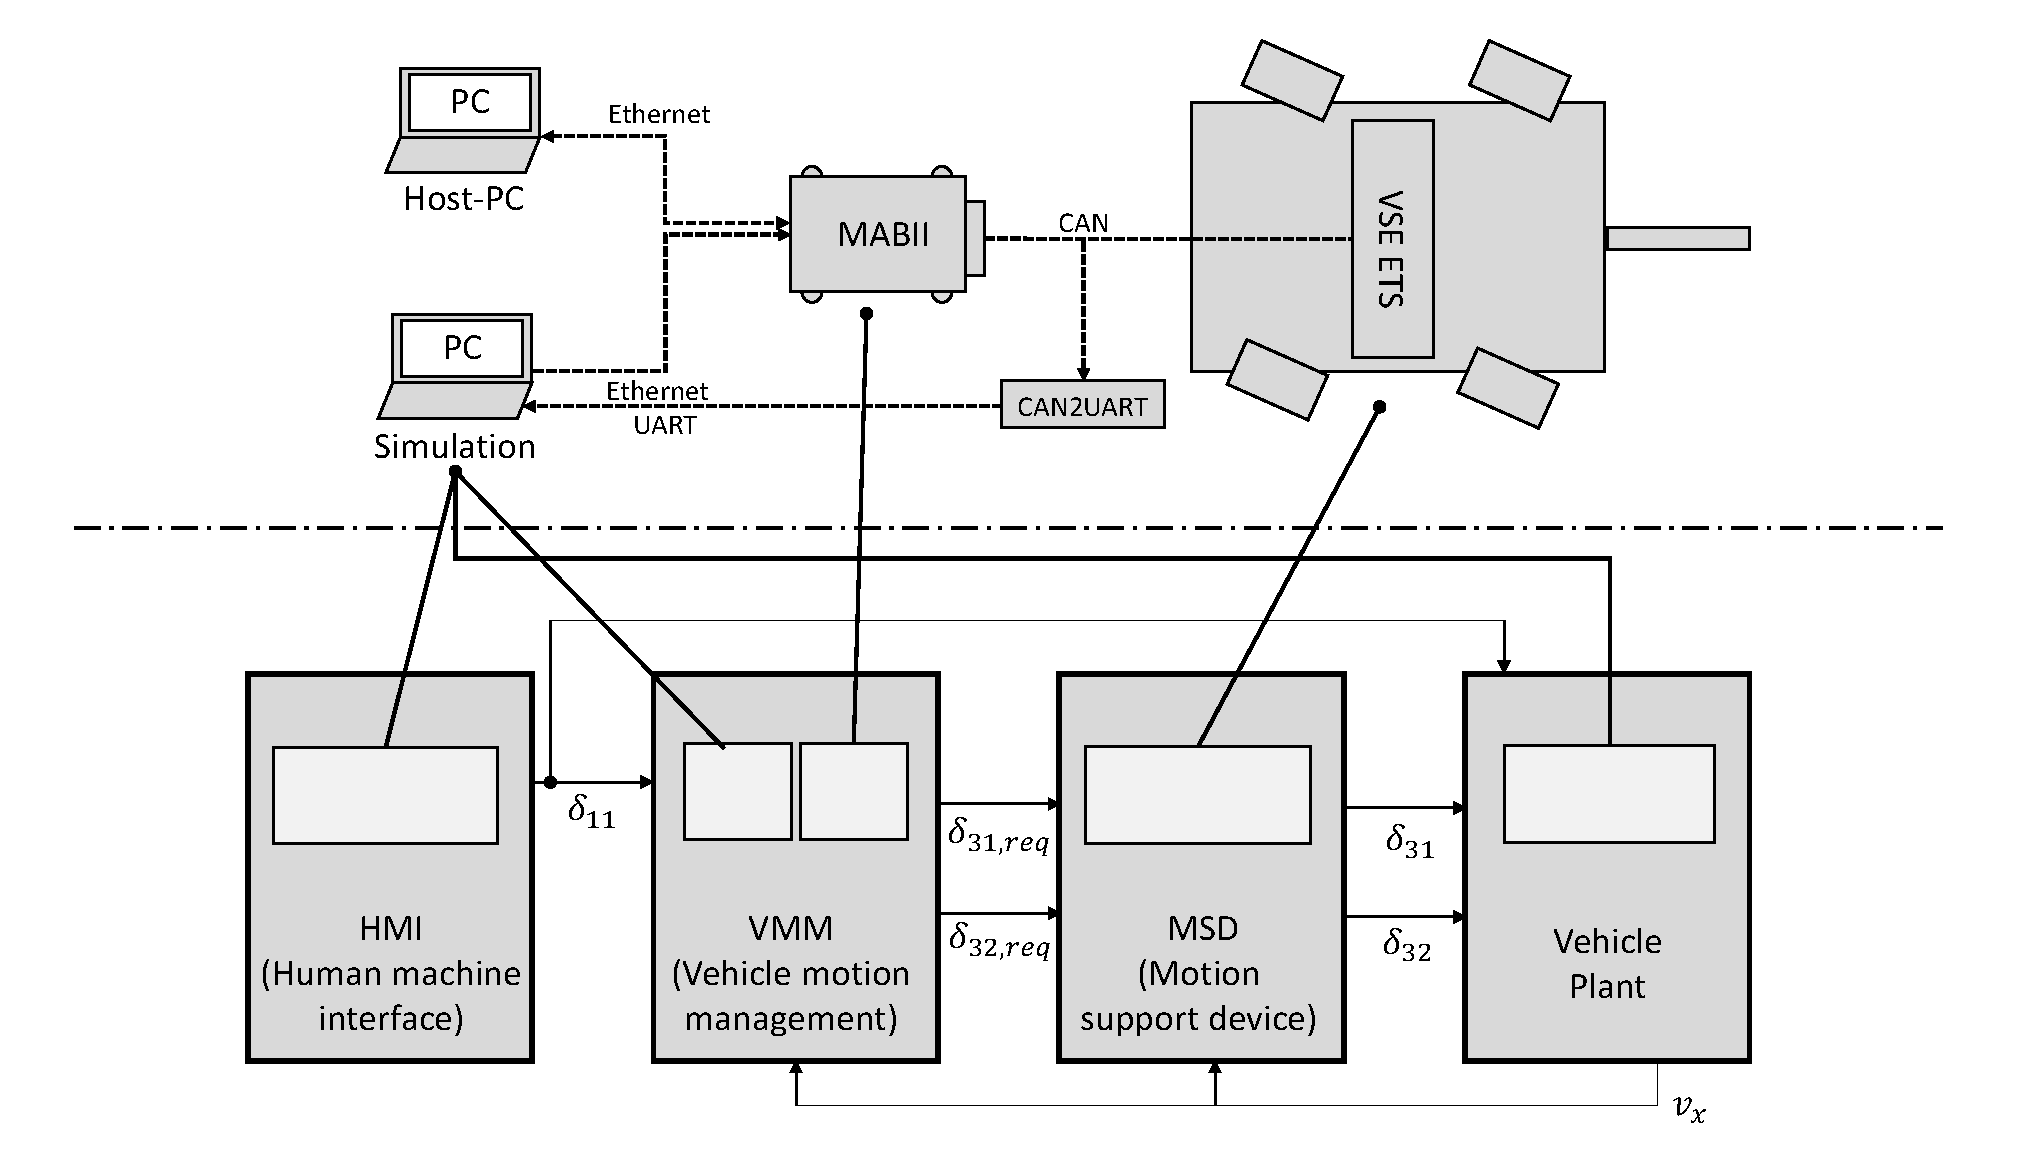
\includegraphics[width=0.8\linewidth]{HIL_overview}
	\caption[Overview of \acrlong{HIL}-simulation, distribution of sub-functions over different physical platforms (top) and correlation to Volvo functionality architecture (bottom)]{Overview of \gls{HIL}-simulation, distribution of sub-functions over different physical platforms (top) and correlation to Volvo functionality architecture (bottom)}
	
	\label{fig:HIL_overview}
\end{figure*}


\section{Delays}

\section{Showcase Maneuver}

To briefly show the general functioning and to give the reader insight into a practical application of the project, a standard driving maneuver was performed on the platform. As an example the U-turn was chosen, for its relevance in everyday driving and the fact that it shows some of the characteristics of \gls{HCT}-combinations distinctively. It was executed at a longitudinal speed of $2m/s$, thus resulting in a turning radius of approx. 16m. To eliminate ensure consistent behaviour over all measurements, the steering-angles of the truck where pre-programmed.


\begin{itemize}
	\item explain off-tracking as a measure 
	\item swept path deviation	
\end{itemize}


\section{RESULTS AND DISCUSSIONS}


\section{RELATED WORKS}

The limitation of this papers were mostly due to time constraints. The 
\section{CONCLUSIONS}



\addtolength{\textheight}{-12cm}   % This command serves to balance the column lengths
                                  % on the last page of the document manually. It shortens
                                  % the textheight of the last page by a suitable amount.
                                  % This command does not take effect until the next page
                                  % so it should come on the page before the last. Make
                                  % sure that you do not shorten the textheight too much.

%%%%%%%%%%%%%%%%%%%%%%%%%%%%%%%%%%%%%%%%%%%%%%%%%%%%%%%%%%%%%%%%%%%%%%%%%%%%%%%%



%%%%%%%%%%%%%%%%%%%%%%%%%%%%%%%%%%%%%%%%%%%%%%%%%%%%%%%%%%%%%%%%%%%%%%%%%%%%%%%%



%%%%%%%%%%%%%%%%%%%%%%%%%%%%%%%%%%%%%%%%%%%%%%%%%%%%%%%%%%%%%%%%%%%%%%%%%%%%%%%%
\section*{APPENDIX}


\section*{ACKNOWLEDGMENT}

This work was mainly carried out during a master-thesis at the department of Applied Mechanics at Chalmers University of Technology, Gothenborg, Sweden. The authors were given great freedom and trust to implement the solutions presented above, for which we are very thankful. 


%%%%%%%%%%%%%%%%%%%%%%%%%%%%%%%%%%%%%%%%%%%%%%%%%%%%%%%%%%%%%%%%%%%%%%%%%%%%%%%%

%References are important to the reader; therefore, each citation must be complete and correct. If at all possible, references should be commonly available publications.



\begin{thebibliography}{99}

\bibitem{c27} M.S. Kati, J. Fredriksson, L. Laine, B. Jacobson,``Performance Improvement for A-double Combination by introducing a Smart Dolly," in Proceedings of the 13th International Heavy Vehicle Transport Technology Symposium, San Luis, Argentina, 2014.

\bibitem{nilsson2015traffic},
	title={On Traffic Situation Predictions for Automated Driving of Long Vehicle Combinations},
	author={Nilsson, Peter},
	year={2015},
	publisher={Chalmers University of Technology}


%\bibitem{c1} G. O. Young, �Synthetic structure of industrial plastics (Book style with paper title and editor),� 	in Plastics, 2nd ed. vol. 3, J. Peters, Ed.  New York: McGraw-Hill, 1964, pp. 15�64.
%\bibitem{c2} W.-K. Chen, Linear Networks and Systems (Book style).	Belmont, CA: Wadsworth, 1993, pp. 123�135.
%\bibitem{c3} H. Poor, An Introduction to Signal Detection and Estimation.   New York: Springer-Verlag, 1985, ch. 4.
%\bibitem{c4} B. Smith, �An approach to graphs of linear forms (Unpublished work style),� unpublished.
%\bibitem{c5} E. H. Miller, �A note on reflector arrays (Periodical style�Accepted for publication),� IEEE Trans. Antennas Propagat., to be publised.
%\bibitem{c6} J. Wang, �Fundamentals of erbium-doped fiber amplifiers arrays (Periodical style�Submitted for publication),� IEEE J. Quantum Electron., submitted for publication.
%\bibitem{c7} C. J. Kaufman, Rocky Mountain Research Lab., Boulder, CO, private communication, May 1995.
%\bibitem{c8} Y. Yorozu, M. Hirano, K. Oka, and Y. Tagawa, �Electron spectroscopy studies on magneto-optical media and plastic substrate interfaces(Translation Journals style),� IEEE Transl. J. Magn.Jpn., vol. 2, Aug. 1987, pp. 740�741 [Dig. 9th Annu. Conf. Magnetics Japan, 1982, p. 301].
%\bibitem{c9} M. Young, The Techincal Writers Handbook.  Mill Valley, CA: University Science, 1989.
%\bibitem{c10} J. U. Duncombe, �Infrared navigation�Part I: An assessment of feasibility (Periodical style),� IEEE Trans. Electron Devices, vol. ED-11, pp. 34�39, Jan. 1959.
%\bibitem{c11} S. Chen, B. Mulgrew, and P. M. Grant, �A clustering technique for digital communications channel equalization using radial basis function networks,� IEEE Trans. Neural Networks, vol. 4, pp. 570�578, July 1993.
%\bibitem{c12} R. W. Lucky, �Automatic equalization for digital communication,� Bell Syst. Tech. J., vol. 44, no. 4, pp. 547�588, Apr. 1965.
%\bibitem{c13} S. P. Bingulac, �On the compatibility of adaptive controllers (Published Conference Proceedings style),� in Proc. 4th Annu. Allerton Conf. Circuits and Systems Theory, New York, 1994, pp. 8�16.
%\bibitem{c14} G. R. Faulhaber, �Design of service systems with priority reservation,� in Conf. Rec. 1995 IEEE Int. Conf. Communications, pp. 3�8.
%\bibitem{c15} W. D. Doyle, �Magnetization reversal in films with biaxial anisotropy,� in 1987 Proc. INTERMAG Conf., pp. 2.2-1�2.2-6.
%\bibitem{c16} G. W. Juette and L. E. Zeffanella, �Radio noise currents n short sections on bundle conductors (Presented Conference Paper style),� presented at the IEEE Summer power Meeting, Dallas, TX, June 22�27, 1990, Paper 90 SM 690-0 PWRS.
%\bibitem{c17} J. G. Kreifeldt, �An analysis of surface-detected EMG as an amplitude-modulated noise,� presented at the 1989 Int. Conf. Medicine and Biological Engineering, Chicago, IL.
%\bibitem{c18} J. Williams, �Narrow-band analyzer (Thesis or Dissertation style),� Ph.D. dissertation, Dept. Elect. Eng., Harvard Univ., Cambridge, MA, 1993. 
%\bibitem{c19} N. Kawasaki, �Parametric study of thermal and chemical nonequilibrium nozzle flow,� M.S. thesis, Dept. Electron. Eng., Osaka Univ., Osaka, Japan, 1993.
%\bibitem{c20} J. P. Wilkinson, �Nonlinear resonant circuit devices (Patent style),� U.S. Patent 3 624 12, July 16, 1990. 






\end{thebibliography}




\end{document}
